\documentclass{beamer}

\definecolor{beaver}{HTML}{8F0000}

\mode<presentation>
{
	\usetheme{Berlin}      % or try Darmstadt, Madrid, Warsaw, ...
	\usecolortheme{beaver} % or try albatross, beaver, crane, ...
	\usefonttheme{default}  % or try serif, structurebold, ...
	\setbeamertemplate{navigation symbols}{}
	\useoutertheme[subsection=false]{smoothbars}
	\setbeamertemplate{itemize item}{\color{beaver}$\blacksquare$}
} 

\usepackage[ngerman]{babel}
\usepackage[utf8x]{inputenc}
\usepackage[T1]{fontenc}
\usepackage{xcolor}

\usepackage{amsmath}
\usepackage{graphicx}


\title{Entwicklung einer Webanwendung zur Annotation spezifischer linguistischer Merkmale in Fließtexten}

\subtitle{Masterarbeit Medieninformatik}
\author{Oliver Brehm}
\institute[Eberhard Karls Universität Tübingen] 
{
	Eberhard Karls Universität Tübingen\\
	Mathematisch-Naturwissenschaftliche Fakultät \\
	Wilhelm-Schickard-Institut für Informatik
}
\date{14. Februar 2018}

\begin{document}
	
\begin{frame}[plain]
	\titlepage
\end{frame}

\begin{frame}{Motivation}
\begin{itemize}
	\item \textbf{Lese- Rechtschreibschwäche}: Weit verbreitete Entwicklungsstörung
	\item Übungstexte mit Hervorhebung von Silben in verschiedenen Farben (Unterstützung bei der Wortdekodierung)
	\item Training der Bewusstheit des Sprachrhythmus (Betonte Silbe)
	\item Webanwendung zur automatischen Erstellung von Übungstexten, Fokus auf User Experience
	\item \textbf{Zielgruppe}: LerntherapeutInnen, LinguistInnen, Eltern betroffener Kinder
\end{itemize}
\end{frame}

\begin{frame}{Eine Webanwendung zur Textannotation}
\centering
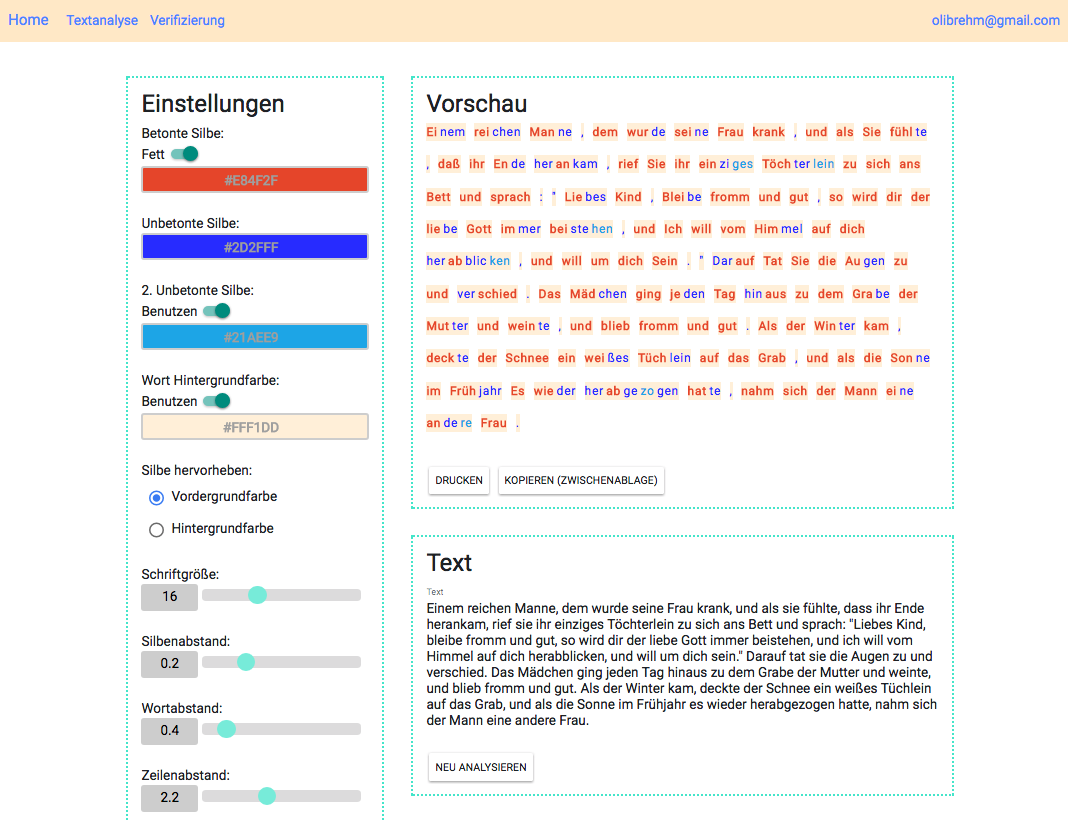
\includegraphics[height=0.8\textheight]{../figures/frontend/textanalyse}
\end{frame}

\section{Grundlagen}
\begin{frame}
	\centering
	\huge{Grundlagen und Forschung}
\end{frame}

\begin{frame}{Linguistische Analyse}
\begin{itemize}
	\item beliebiger Eingabetext
	\item Parser/Tokenizer (Spacy mit Python)
	\item Tagging (Part-of-Speech, Lemma)
\end{itemize}
\vfill
\centering
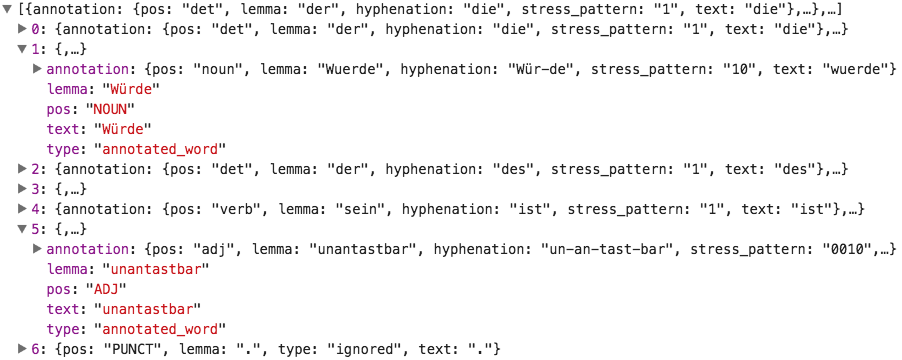
\includegraphics[width=1.05\textwidth]{../figures/json}
\end{frame}

\begin{frame}{Wortdatenbank}
\textbf{Silbentrennung und Wortbetonung gesucht}
\begin{itemize}
	\item Silbentrennung aus Hyphenator (Pyphen)
	\item \textbf{Wortbetonung}: Lexikon CELEX2 als Goldstandard
	\item Bestimmung der Betonung aus Phonologischer Darstellung (z.b. \textit{antizipiert | \&n-ti-=i-'pirt})
	\item Nicht alle Wörter (mit Flexionsformen) enthalten
	\item Generieren von Vorschlägen bei unbekannten Wörtern
	\item Text-to-Speech Systeme (z.B. MARY) für Wortbetonung
\end{itemize}
\end{frame}

\section{Entwicklung der Anwendung}
\begin{frame}
\centering
\huge{Entwicklung der Anwendung}
\end{frame}

\begin{frame}{Aufbau der Anwendung}
	\begin{itemize}
		\item Anforderungsanalyse mit Expertengesprächen
	\end{itemize}

	\centering
	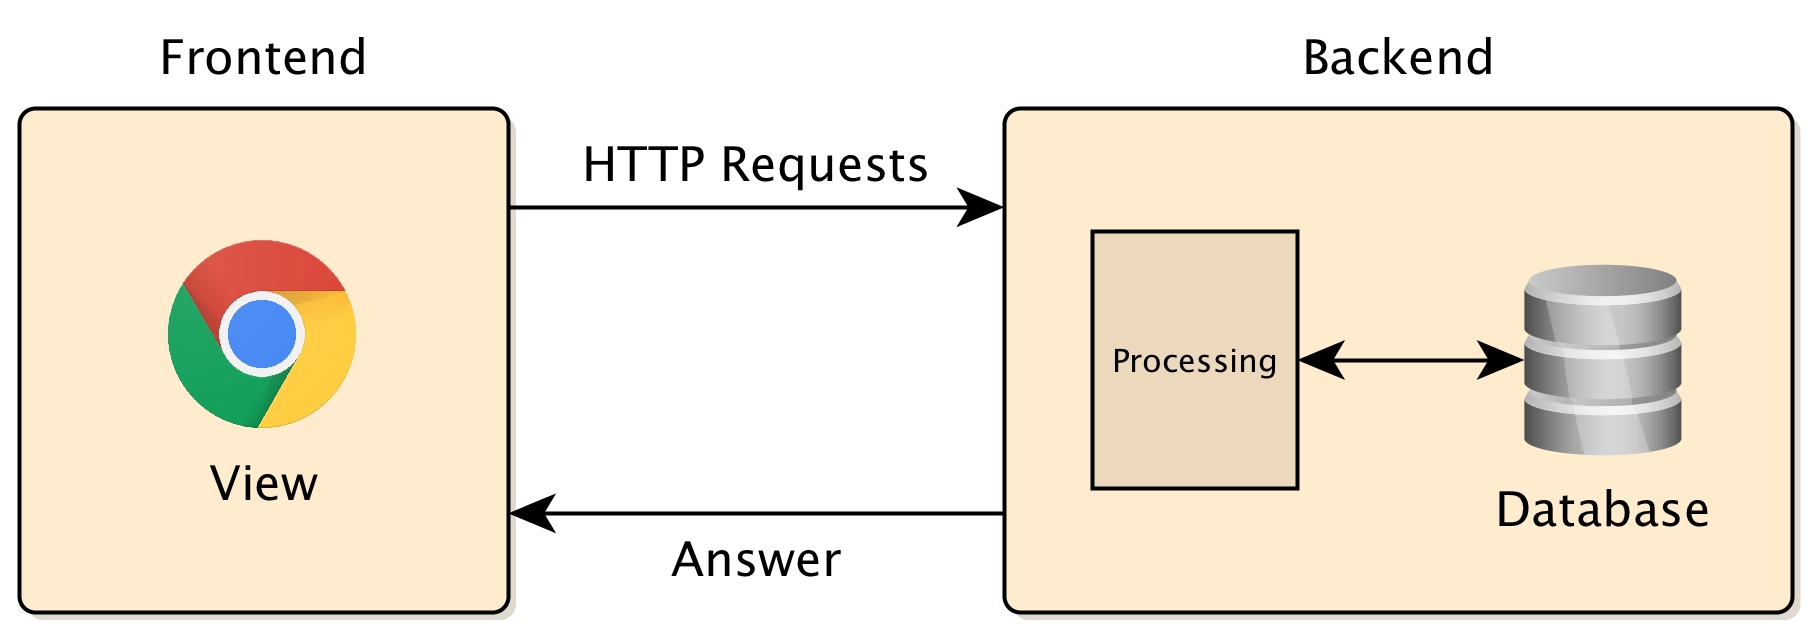
\includegraphics[width=0.85\textwidth]{../figures/frontendbackend}\\
	
	\begin{itemize}
		\item RESTful API mit Python und Flask
		\item Wort- und User-Datenbanken (SQLite)
	\end{itemize}
\end{frame}

\begin{frame}{Backend}
	\centering
	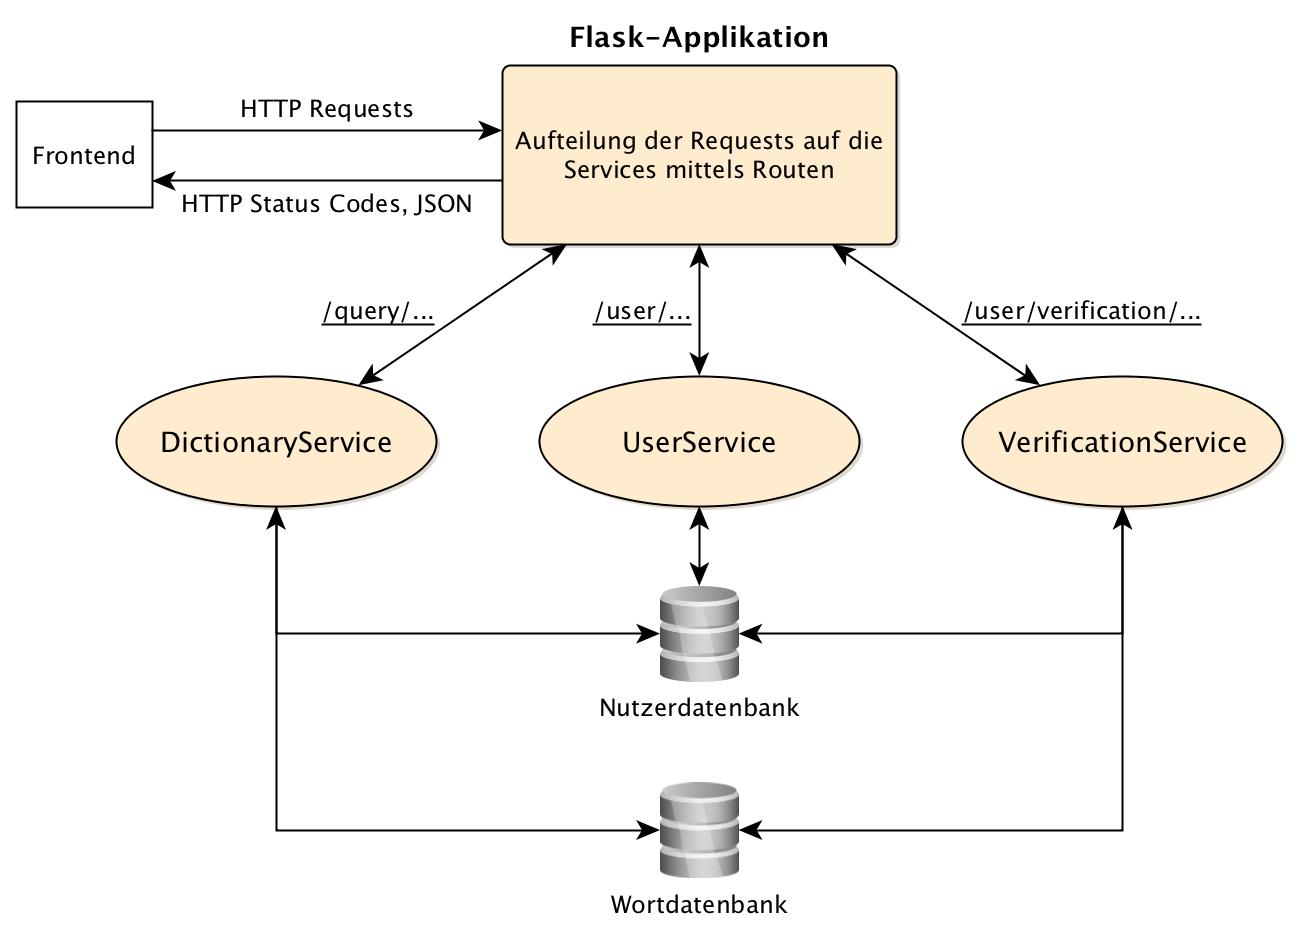
\includegraphics[width=0.95\textwidth]{../figures/backend}
\end{frame}

\begin{frame}{Frontend}
\begin{itemize}
	\item Single-Page-Application
	\item AngularDart Framework
	\item Datenmodell in Dart Klassen
	\item HTML/CSS Templates mit Data Binding
\end{itemize}
\centering
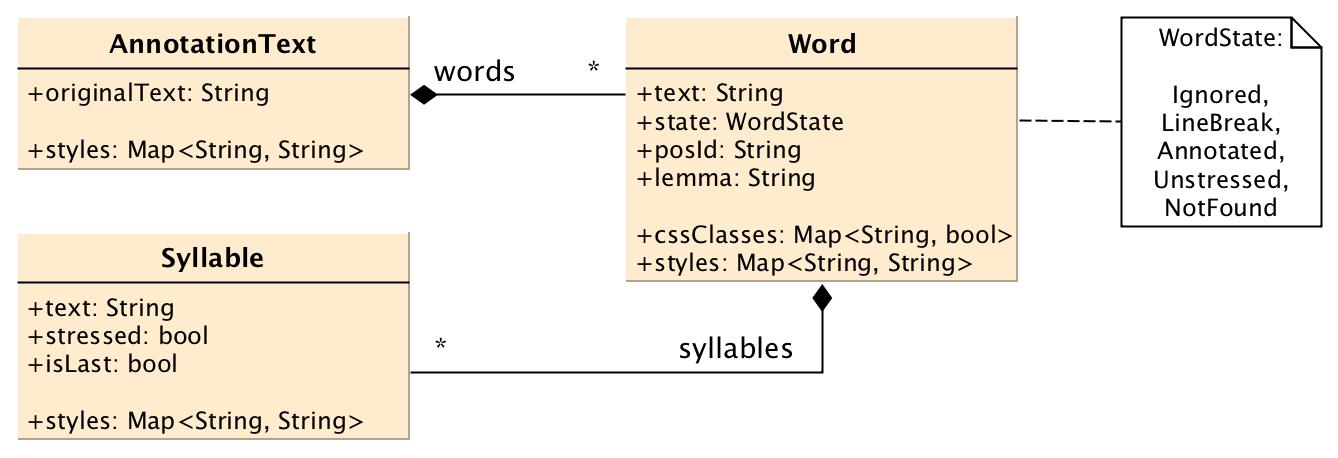
\includegraphics[width=0.95\textwidth]{../figures/frontend/uml-annotationtext}
\end{frame}

\begin{frame}{Wort-Verifizierung}
\begin{itemize}
	\item Manuelle Eingabe von Silbentrennung und Wortbetonung mit Vorschlägen
	\item Übertragung in die Wortdatenbank nach Abstimmung
	\item Crowdsourcing nach dem Mehrheitsprinzip
\end{itemize}
\centering
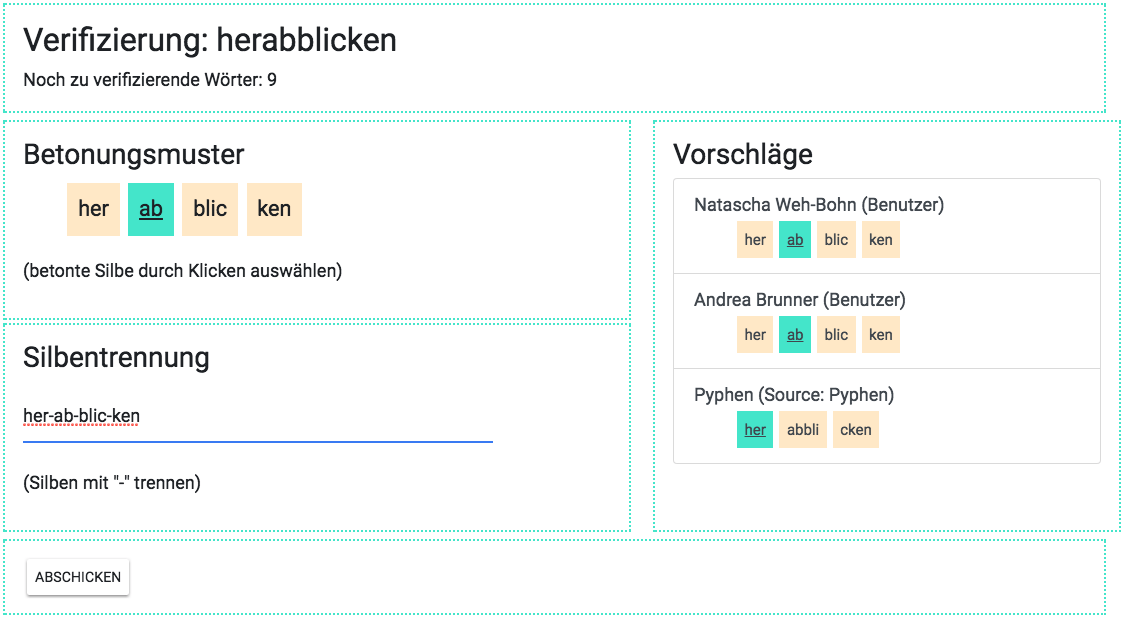
\includegraphics[width=0.75\textwidth]{../figures/frontend/verifizierung}
\end{frame}

\section{Evaluation}
\begin{frame}
\centering
\huge{Evaluation}
\end{frame}

\begin{frame}{Ergebnisse der Textannotation}
\begin{columns}[t]
	\column{.5\textwidth}
	\centering
	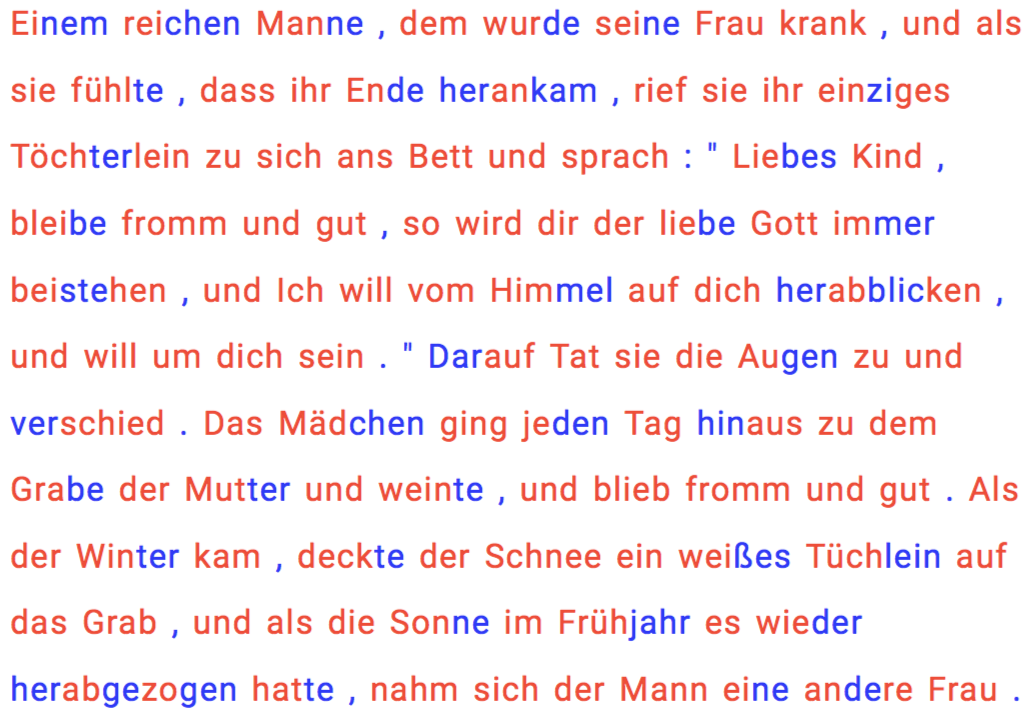
\includegraphics[width=5.5cm]{../figures/evaluation/pre-annotation1}\\
	[0.5cm]
	Einfache, abwechselnde Darstellung
	\column{.5\textwidth}
	\centering
	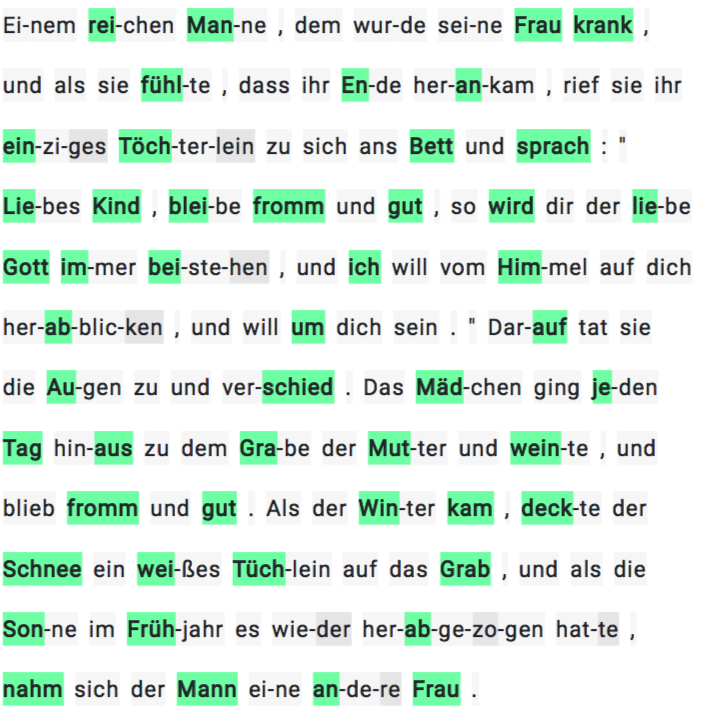
\includegraphics[width=5.5cm]{../figures/evaluation/pre-annotation3}\\
	[0.5cm]
	Andere Farben, manuelle Aktivierung der Betonung
\end{columns}
\end{frame}

\begin{frame}{Nutzertest}
\begin{itemize}
	\item Fünf aufeinanderfolgende Szenarien
	\item Interview mit \textit{Thinking Aloud}
	\item Zusätzlich \textit{After Scenqrio Questionnaire} für quantitative Daten
	\item Pilottest
	\item Sieben ProbandInnen aus zwei Gruppen
\end{itemize}
\end{frame}

\begin{frame}{Ergebnisse der Szenarien}
\begin{columns}[t]
	\column{.5\textwidth}
	\centering
	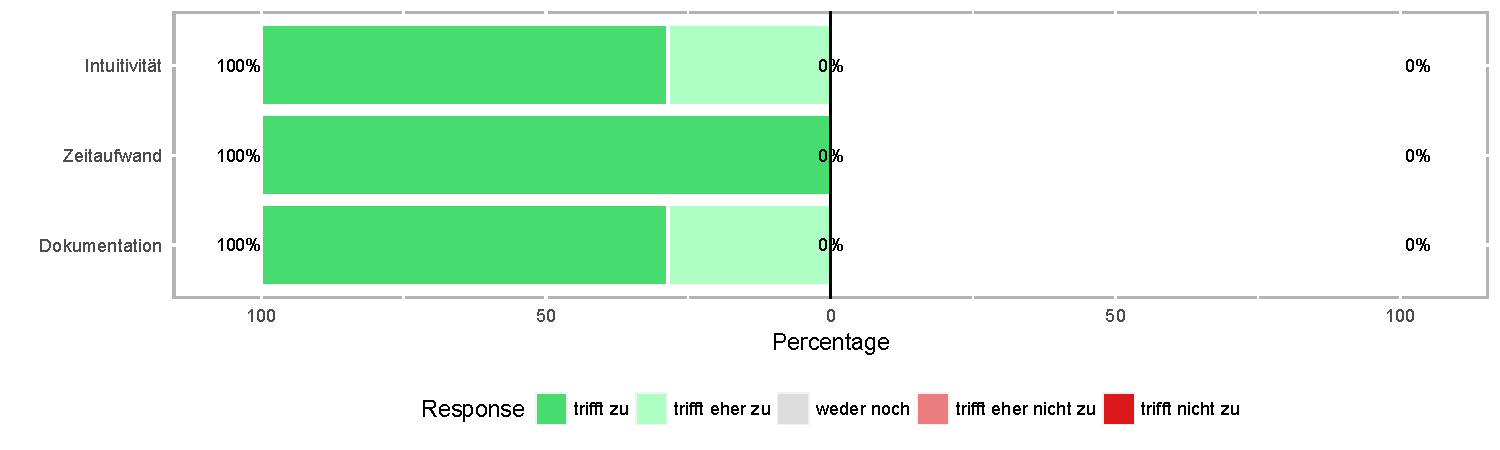
\includegraphics[width=5.5cm]{../figures/evaluation/scenario1}\\
	1: Nutzerkonto\\
	[1.5cm]
	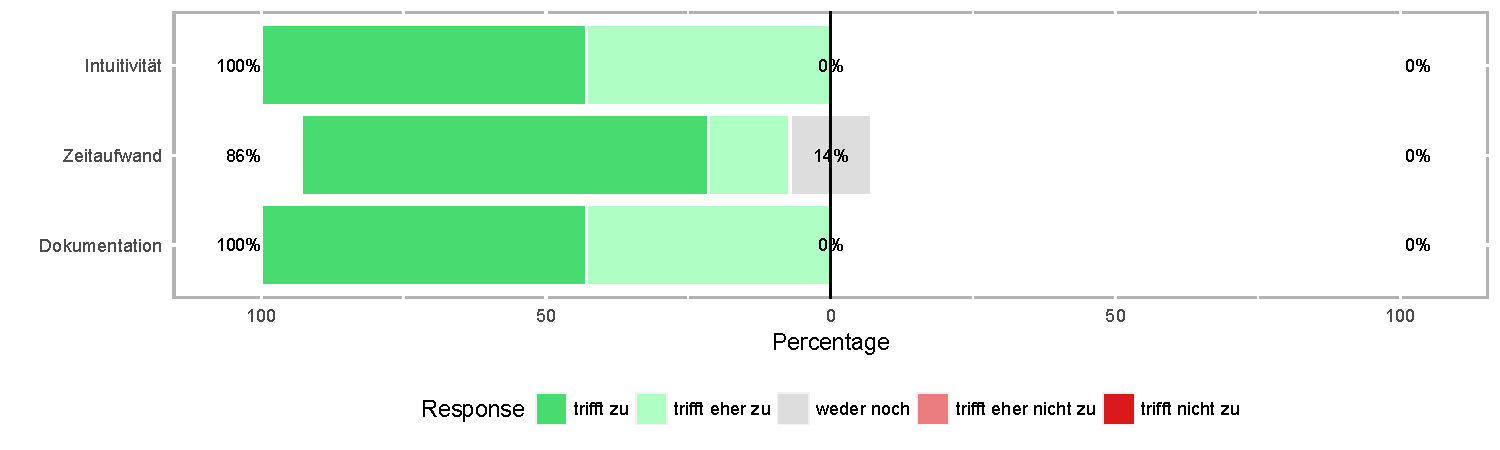
\includegraphics[width=5.5cm]{../figures/evaluation/scenario2}\\
	2: Textanalyse
	\column{.5\textwidth}
	\centering
	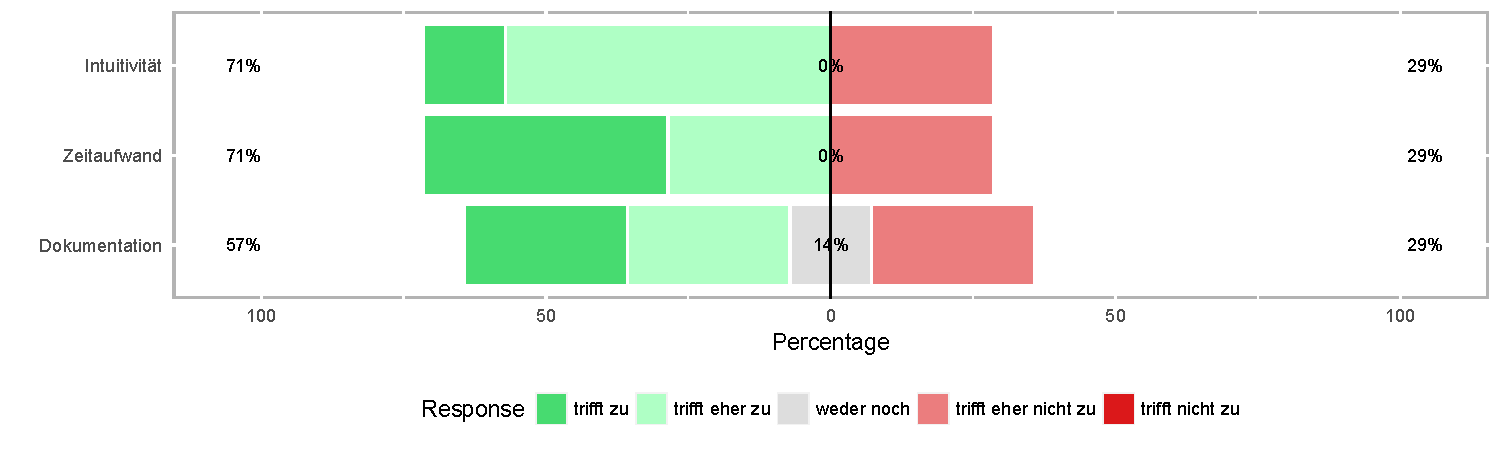
\includegraphics[width=5.5cm]{../figures/evaluation/scenario3}\\
	3: Annotationsvorlagen\\
	[1.5cm]
	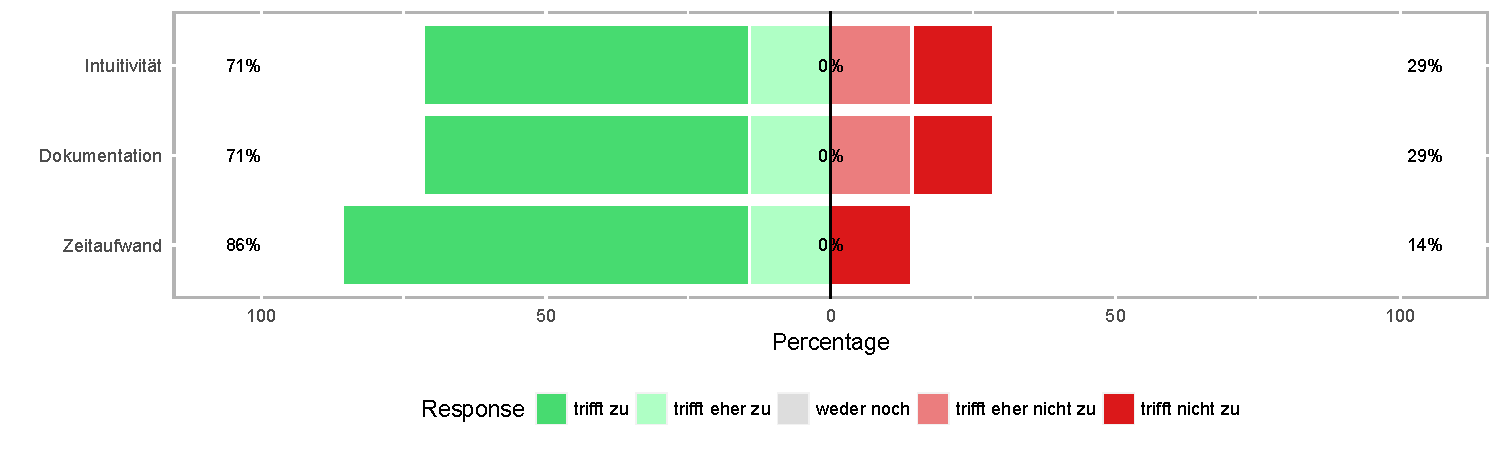
\includegraphics[width=5.5cm]{../figures/evaluation/scenario4}\\
	4: Texte wiederverwenden
\end{columns}
\end{frame}

\begin{frame}{Fazit}
\begin{itemize}
	\item Automatische Erstellung von Übungstexten, Arbeitserleichterung
	\item Erweiterbare Wortdatenbank durch Crowdsourcing
	\item Intuitive Bedienbarkeit
	\item Erweiterungen möglich (Modul für SchülerInnen, mobile App...)
\end{itemize}
\end{frame}

\begin{frame}[plain]
\centering
\huge{Danke für die Aufmerksamkeit!}
\\
[1cm]
\huge{\color{beaver}{$\rightarrow$ Fragen und Demo}}
\end{frame}

\end{document}